%==================================================================%
% Author : Doe Doe, John                                           %
%          S�nchez Barreiro, Pablo                                 %
% Version: 1.0, dd/mm/yyyy                                         %                   %                                                                  %
% Memoria del Proyecto Fin de Carrera                              %
% Archivo ra�z                                                     %
%==================================================================%

\documentclass[a4paper,11pt]{itsas_pfc}

%=====================================================================%
%                       My imported packages                          %
%=====================================================================%
\usepackage[latin1]{inputenc}
\usepackage{longtable}
\usepackage{array}
\usepackage{url}
\usepackage{amsfonts}
\usepackage[spanish,activeacute]{babel}

% Esto se a�ade porque a alg�n gracioso le apetec�a que la fuente
% de la portada fuese Arial
\usepackage[T1]{fontenc}
\usepackage[scaled]{uarial}

% File with main configuration
\input{config/pfc_options.tex}

% File with some names
%
% This file has a list of internal names (variables) of LaTeX,
% of which you can change the value. For example, you can make
% chapters read "Section" instead of "Chapter".
%
\renewcommand\bibname{References}                 % thus Bibliography will read "References"
%\renewcommand{\tablename}{xxx}                   % name below each table (xxx 1: bla-bla-bla)
%\renewcommand{\figurename}{xxx}                  % name below each figure (xxx 1: bla-bla-bla)
%\renewcommand{\listtablename}{yyy}               % name for table of tables
%\renewcommand{\listfigurename}{yyy}              % name for table of figures


%=====================================================================%
%                           Authoring's details                          %
%=====================================================================%
\newcommand{\myname}{John Doe Doe}  % name of author
\newcommand{\myboss}{Pablo S�nchez Barreiro} % name of supervisor
\newcommand{\thesistitle}{T�tulo del Proyecto Fin de Carrera}

\newcommand{\englishtitle}{Master Thesis Title}
												  % work title
\newcommand{\worktype}{Proyecto Fin de Carrera}   % work type
\newcommand{\logo}{images/uc.eps}            % logo file (e.g. for the cover)

%=====================================================================%
%                     Definition of my own commands                   %
%=====================================================================%
\newcommand{\nota}[1]{\color{red}$\ll$#1$\gg$\color{black}}
\newcommand{\imp}[1]{{\small{\sf #1}}}
\newcommand{\stereotype}[1]{$\ll${\small{\sf #1}}$\gg$}
\newcommand{\todo}[1]{\color{red}$\ll$TODO: #1$\gg$\color{black}}

\setcounter{minitocdepth}{1}

\begin{document}

% Cover page
%
% This file produces the first page of the PFC/Thesis, featuring
% the title, your name, supervisor's name and so forth.
%
% Most, if not all, content in this page is included via commands
% (e.g. \thesistitle) that have been defined in Config/pfc_options.tex
%
% Edit to your liking.
%

\thispagestyle{empty} % don't print neither page number nor headers nor footers.

%
% Use \tb to place the various items in the page. Usage:
%
% \tb{w}{h}{v}{t}
%
% where:
%
% w = paragraph width of text box (1.0 = page width)
% h = horizontal position of the center of text box (0.0 = left, 1.0 = right)
% v = vertical position of the center of text box (0.0 = top, 1.0 = bottom)
% t = text to put inside text box
%
\tb{0.8}{0.50}{0.100}{\large FACULTAD DE CIENCIAS}
\tb{0.8}{0.50}{0.130}{\Large UNIVESIDAD DE CANTABRIA}
\tb{0.8}{0.50}{0.250}{
	
\includegraphics[width=0.30\columnwidth]{images/ingInformatica.eps} \ \ \ \ \
}
\tb{0.8}{0.50}{0.390}{\LARGE \worktype}    % whether this is a PFC or a Thesis
\tb{0.8}{0.50}{0.500}{\Huge \thesistitle}  % title of the work
\tb{0.8}{0.50}{0.600}{\LARGE (\englishtitle)}  % title of the work
\tb{0.8}{0.50}{0.700}{\Large Para acceder al T�tulo de \\
					  INGENIERO EN INFORM�TICA}   % the name of the supervisor
\tb{0.2}{0.70}{0.850}{\begin{tabular}{r}
\Large Autor: \myname \\
\Large Julio 2011 \\
\end{tabular}}

\ \clearpage                       % end page here
\thispagestyle{empty} \ \clearpage % blank page


\begin{tabular}{p{.15\textwidth}p{.50\textwidth}p{.15\textwidth}}
	\includegraphics[width=\linewidth]{\logo} & 
	\begin{center}FACULTAD DE CIENCIAS\end{center} & \\
\end{tabular}

\vspace{-15pt}

\begin{center}
INGENIER�A EN INFORM�TICA
\end{center}

\begin{center}
CALIFICACI�N DEL PROYECTO FIN DE CARRERA
\end{center}

\begin{tabular}{p{0.25\textwidth}p{0.75\textwidth}}
Realizado por:    & \myname \\ 
Director del PFC: & \myboss \\
T�tulo:           & \thesistitle  \\   
Title:            & \englishtitle \\  
\end{tabular}


Presentado a examen el d�a: 

\begin{center}
para acceder al T�tulo de \\ 
INGENIERO EN INFORM�TICA
\end{center}

\underline{Composici�n del Tribunal:} \\

\begin{tabular}{ll}
Presidente (Apellidos, Nombre): & \\
Secretario (Apellidos, Nombre): & \\
Vocal (Apellidos, Nombre): & \\
Vocal (Apellidos, Nombre): & \\
Vocal (Apellidos, Nombre): & \\
\end{tabular}

\ \\

Este Tribunal ha resuelto otorgar la calificaci�n de: ......................................

\begin{center}
\begin{tabular}{cc}
& \\
& \\
& \\
\ \ \ \ \ \ \ \ \ \ \ \
Fdo.: El Presidente 
\ \ \ \ \ \ \ \ \ \ \ \ &  
\ \ \ \ \ \ \ \ \ \ \ \
Fdo.: El Secretario  
\ \ \ \ \ \ \ \ \ \ \ \ \\
& \\
& \\
& \\
Fdo.: Vocal \ \ \ \ \ \          &         Fdo.: Vocal \ \ \ \ \ \ \\
& \\
& \\
& \\
Fdo.: Vocal \ \ \ \ \ \          &         Fdo.: El Director del PFC \ \ \ \ \ \  \\
\end{tabular}
\end{center}

\thispagestyle{empty} \



% reset page numbering
\input{config/begin.tex}

% acknowledgement
\cdpchapter{Agradecimientos}

TODO: Aqu� se suelen poner agradecimientos si uno quiere y dedicatorias.
 % acknowledgements

% Preface
%\input{introduction/preface-lff.tex}   % preface

% Toc
\input{config/toc.tex}

\input{Config/headers.tex}

\input{config/chapters.tex}

% Cap�tulo 1: Introducci�n
\todo{Cap�tulo 1: Introducci�n al proyecto}
%==================================================================%
% Author : Doe Doe, John                                           %
%          S�nchez Barreiro, Pablo                                 %
% Version: 1.0, dd/mm/yyyy                                         %                   %                                                                  %
% Memoria del Proyecto Fin de Carrera                              %
% Introducci�n, archivo ra�z                                       %
%==================================================================%

%%% Schema to write a paper introduction
%% Description of Purpose
	% What problem, issue or question does this research address ?
		%
	% What limitations or failings of current understanding, knowledge, method,
	% or technologies does this research resolve ?
		%
	% What is the significance of the problem issue or question ?
		%
%% Goal statement
	% What new understanding, knowledge, methods or technologies will this
	% research generate ?
		%
	% How this address the purpose of the work ?
		%
%% Approach
	% What experiments, prototypes or studies will be done to achieve the stated % goal ?
		%
	% How will achievement or contribution of the research be demonstrated or validated ?
		%

\chapterheader{Introduction}{Introduction}
\label{chap:introduction}

% Introducci�n al cap�tulo

\chaptertoc

\section{Introducci�n}
\label{sec:intr:introduction}

TODO: Siguiendo el esquema que aparece arriba, escribir la introducci�n

\section{Motivaci�n and Contribuciones}
\label{sec:intr:motivation}

TODO: Esta secci�n es m�s para tesis doctorales que para proyectos fin de carrera. La dejamos de momento pero se podr�a eliminar

\section{Visi�n General del Proyecto}
\label{sec:intr:overview}

TODO: Esto est� bien dejarlo, pero tambi�n es suprimible

\section{Estructura del Documento}
\label{sec:intr:organization}

Esto es una especie de �ndice ampliado y se deja, suele ser bastante �til para que el que est� vago se lea esto y se acabe el problema.





 % Chapter 1

% Cap�tulo 2: Resumen del Estado del Arte
\todo{Cap�tulo 2: Antecedentes o Estado del Arte}
%%==================================================================%%
%% Author : Tejedo Gonz�lez, Daniel                                 %%
%%          S�nchez Barreiro, Pablo                                 %%
%% Version: 1.0, 18/11/2012                                         %%                   %%                                                                  %%
%% Memoria del Proyecto Fin de Carrera                              %%
%% Antecedentes, archivo ra�z                                       %%
%%==================================================================%%

\chapterheader{Antecedentes}{Antecedentes}
\label{chap:background}

Este cap�tulo trata de describir a grandes rasgos las t�cnicas, tecnolog�as y herramientas utilizadas para el desarrollo del presente Proyecto Fin de Carrera. En primer lugar, se introducir� el caso de estudio que se utilizar� de forma recurrente a lo largo del proyecto, que es una l�nea de productos software para software de control para hogares inteligentes. Para ello se describen en primer lugar diversos conceptos relacionados el dominio del proyecto, como son las l�neas de productos software y los �rboles de caracter�sticas. A continuaci�n, se describen dos principales herramientas de Ingenier�a de Lenguajes Dirigida por Modelos utilizadas: \emph{Ecore} y \emph{EMFText}. Por �ltimo, se describe brevemente la arquitectura de plugins de Eclipse, dado que nuestro proyecto deb�a integrarse en dicho entorno.

\chaptertoc

\section{Caso de Estudio: Software para Hogares Inteligentes}
\label{sec:back:spl}
%%==================================================================%%
%% Author : Perez Ruiz, Alejandro                                   %%
%% Author : Pablo S�nchez                                           %%
%% Version: 1.1, 13/06/2011                                         %%
%%                                                                  %%
%% Memoria del Proyecto Fin de Carrera                              %%
%% Planificacion/CasoEstudio                                        %%
%%==================================================================%%

El objetivo �ltimo del presente proyecto es la construcci�n de una l�nea de productos software sobre la plataforma .NET para hogares automatizados y/o inteligentes.

%%===========================================================================%%
%% NOTA(Pablo): Dado el contexto del proyecto, este p�rrafo no interesa      %%
%%===========================================================================%%
%%
%% Se ha elegido este dominio de aplicaci�n por ser un dominio donde el uso
%% de un enfoque basado en L�neas de Productos Software se hace casi
%% imperativo, debido a la gran variabilidad existente en estos productos.
%% Esta  variabilidad se debe tanto a motivos de hardware, dado que los
%% dispositivos a ser controlados e interconectados pueden variar enormemente,
%% como funcionales, dado que existen multitud de funcionalidades que se pueden
%% ofrecer de manera opcional o alternativa al usuario, no siendo necesario que
%% un determinado hogar las posea todas ellas.
%%
%%===========================================================================%%

El objetivo de estos hogares es aumentar la comodidad y seguridad de sus habitantes, as� como hacer un uso m�s eficiente de la energ�a consumida. Los ejemplos m�s comunes de tareas automatizadas dentro de un hogar inteligente son el control de las luces, ventanas, puertas, persianas, aparatos de fr�o/calor, as� como otros dispositivos, que forman parte de un hogar. Un hogar inteligente tambi�n busca incrementar la seguridad de sus habitantes mediante sistemas automatizados de vigilancia y alerta de potenciales situaciones de riesgo. Por ejemplo, el sistema deber�a encargarse de detecci�n de humos o de la existencia de ventanas abiertas cuando se abandona el hogar.

El funcionamiento de un hogar inteligente se basa en el siguiente esquema: (1) el sistema lee datos o recibe datos de una serie de sensores; (2) se procesan dichos datos; y (3) se activan los actuadores para realizar las acciones que correspondan en funci�n de los datos recibidos de los sensores.

Todos los sensores y actuadores se comunican a trav�s de un dispositivo especial denominado puerta de enlace (\emph{Gateway}, en ingl�s). Dicho dispositivo se encarga de coordinar de forma adecuada los diferentes dispositivos existentes en el hogar, de acuerdo a los par�metros y preferencias especificados por los habitantes del mismo. Los habitantes del hogar se comunicar�n con la puerta de enlace a trav�s de una interfaz gr�fica.
Este proyecto tiene como objetivo el desarrollo de un hogar inteligente como una l�nea de productos software, con un n�mero variable de plantas y habitaciones. El n�mero de habitaciones por planta es tambi�n variable. La l�nea de productos deber� ofrecer varios servicios, que podr�n ser opcionalmente incluidos en la instalaci�n del software para un un hogar determinado. Dichos servicios se clasifican en funciones b�sicas y complejas, las cuales describimos a continuaci�n.

\paragraph{Funciones b�sicas} \ \\

\begin{enumerate}
\item \emph{Control autom�tico de luces:} Los habitantes del hogar deben ser capaces de encender, apagar y ajustar la intensidad de las diferentes luces de la casa. El n�mero de luces por habitaci�n es variable. El ajuste debe realizarse especificando un valor de intensidad.
\item \emph{Control autom�tico de ventanas:} Los residentes tienen que ser capaces de controlar las ventanas autom�ticamente. De tal modo que puedan indicar la apertura de una ventana desde las interfaces de usuario disponibles.
\item \emph{Control autom�tico de persianas:} Los habitantes podr�n subir y bajar las persianas de las ventanas de manera autom�tica.
\item \emph{Control autom�tico de temperatura:} El usuario ser� capaz de ajustar la temperatura de la casa. La temperatura se medir� siempre en grados celsius.
\end{enumerate}

\paragraph{Funciones complejas} \ \\

\begin{enumerate}
\item \emph{Control inteligente de energ�a:} Esta funcionalidad trata de coordinar el uso de ventanas y aparatos de fr�o/calor para regular la temperatura interna de la casa de manera que se haga un uso m�s eficiente de la energ�a. Por ejemplo, si se recibe la orden de calentar la casa, a la vez que se activan los radiadores se cerrar�n las ventanas para evitar las p�rdidas de calor.
\item \emph{Presencia simulada:} Para evitar posibles robos, cuando los habitantes abandonen la casa por un periodo largo de tiempo, se deber� poder simular la presencia de personas en las casas. Hay dos opciones de simulaci�n (no exclusivas):
	\begin{enumerate}
	\item \emph{Simulaci�n de las luces:} Las luces se deber�n apagar y encender para simular la presencia de habitantes en la casa.
	\item \emph{Simulaci�n de persianas:} Las persianas se deber�n subir y bajar autom�tica para simular la presencia de individuos dentro de la casa.
	\end{enumerate}
\end{enumerate}

Todas estas funciones son opcionales. Las personas interesadas en adquirir el sistema podr�n incluir en una instalaci�n concreta de este software el n�mero de funciones que ellos deseen. La siguiente secci�n describe la planificaci�n general realizada para desarrollar este caso de estudio.


\section{L�neas de producto software}
\label{sec:back:spl}
%=============================================================================%
% Author : Alejandro P�rez Ruiz                                               %
% Author : Pablo S�nchez Barreiro                                             %
% Version: 1.1, 10/06/2011                                                    %
% Master Thesis: Background/Software Product Lines                            %
%=============================================================================%

El objetivo de una \emph{l�nea de productos software}~\cite{pohl:2005,kakola:2006} es crear una infraestructura adecuada a partir de la cual se puedan derivar, tan autom�ticamente como sea posible, productos concretos pertenecientes a una familia de productos software. Una familia de productos software es un conjunto de aplicaciones software similares, que por tanto comparten una serie de caracter�sticas comunes, pero que tambi�n presentan variaciones entre ellos.

Un ejemplo cl�sico de familia de productos software es el software que se encuentra instalado por defecto en un tel�fono m�vil. Dicho software contiene una serie de facilidades comunes, tales como agenda, recepci�n de llamadas, env�o de mensajes de texto, etc. No obstante, dependiendo de las capacidades y la gama del producto, �ste puede presentar diversas funcionalidades opcionales, tales como env�o de correos electr�nicos, posibilidad de conectarse a Internet mediante red inal�mbrica, radio, etc.

La idea de una l�nea de productos software es proporcionar una forma automatizada y sistem�tica de construir productos concretos dentro de una familia de productos software mediante la simple especificaci�n de qu� caracter�sticas deseamos incluir dentro de dicho producto. Esto representa una alternativa al enfoque tradicional de desarrollo software, el cual se basaba simplemente en seleccionar el producto m�s parecido dentro de la familia al que queremos construir y adaptarlo manualmente.

El proceso de creaci�n de l�neas de producto software conlleva dos fases: \emph{ingenier�a del dominio} (en ingl�s,  \emph{Domain Engineering}) e \emph{ingenier�a de aplicaci�n} (en ingl�s, \emph{Application Engineering}) (laFfigura~\ref{back:fig:domainAplicEng} ilustra el proceso para ambas fases). La \emph{ingenier�a del dominio} tiene como objetivo la creaci�n de la infraestructura o arquitectura de la l�nea de productos, la cual permitir� la r�pida, o incluso autom�tica, construcci�n de sistemas software espec�ficos pertenecientes a la familia de productos. La \emph{ingenier�a de aplicaci�n} utiliza la infraestructura creada anteriormente para crear aplicaciones espec�ficas adaptadas a las necesidades de cada usuario en concreto.

\begin{figure}[!tb]
  \centering
	\includegraphics[width=.95\linewidth]{background/domainAplicationEngineering.eps} \\
  \caption{Proceso de desarrollo de una l�nea de productos software}
  \label{back:fig:domainAplicEng}
\end{figure}

En la fase de ingenier�a del dominio, el primer paso a realizar ser�a un an�lisis de qu� caracter�sticas de la familia de productos son variables y por qu� y c�mo son variables. Esta parte es la que se conoce como \emph{an�lisis o especificaci�n de la variabilidad} (Figura~\ref{back:fig:domainAplicEng}, punto 1). A continuaci�n, se ha de dise�ar una arquitectura o marco de trabajo para la familia de productos software que permita soportar dichas variaciones. Esta actividad se conoce como \emph{realizaci�n o dise�o de la variabilidad} (Figura~\ref{back:fig:domainAplicEng}, punto 2). El siguiente paso es establecer una serie de reglas que especifiquen como hay que instanciar la arquitectura previamente creada de acuerdo con las caracter�sticas seleccionadas por cada cliente. Esta fase es la que se conoce como \emph{correspondencia entre especificaci�n y dise�o de la variabilidad} (Figura~\ref{back:fig:domainAplicEng}, punto 3).

En la fase de ingenier�a de aplicaci�n, se crear�a una \emph{configuraci�n}, que no es m�s que una selecci�n de caracter�sticas que un usuario desea incluir en su producto (Figura~\ref{back:fig:domainAplicEng}, punto 4). En el caso ideal, usando esta configuraci�n, deber�amos poder ejecutar las reglas de correspondencia entre especificaci�n y dise�o de la variabilidad para que la arquitectura creada en la fase de ingenier�a del dominio se adaptase autom�ticamente generando un producto concreto espec�fico acorde a las necesidades concretas del usuario (Figura~\ref{back:fig:domainAplicEng}, punto 5). En caso no ideal, dichas reglas de correspondencia deber�n ejecutarse a mano, lo cual suele ser un proceso tedioso, largo, repetitivo y propenso a errores.

Este proyecto se centra en la primera etapa de este proceso de desarrollo, es decir en el an�lisis de la variabilidad de una familia de productos software mediante �rboles de caracter�sticas. La siguiente secci�n proporciona una breve pero completa descripci�n acerca del funcionamiento de los �rboles de caracter�sticas.


\section{�rboles de caracter�sticas}
\label{sec:back:fmodels}
%%==================================================================%%
%% Author : Tejedo Gonz�lez, Daniel                                 %%
%%          S�nchez Barreiro, Pablo                                 %%
%% Version: 1.0, 18/11/2012                                         %%                   %%                                                                  %%
%% Memoria del Proyecto Fin de Carrera                              %%
%% Antecedentes, �rboles de caracter�sticas                                    %%
%%==================================================================%%

El objetivo de las l�neas de productos software es crear la infraestructura para la r�pida  producci�n de sistemas software para un segmento de mercado espec�fico, donde estos sistemas software son similares, y aunque comparten un subconjunto de caracter�sticas comunes, tambi�n presentan variaciones entre ellos ~\ref{} ~\ref{} ~\ref{} ~\ref{}.

El principal logro en las l�neas de productos software es, construir productos espec�ficos lo m�s autom�ticamente posible a partir de un conjunto de elecciones y decisiones adoptadas sobre un modelo com�n, conocido como modelo de referencia, que representa la familia completa de productos que la l�nea de productos software cubre.

El desarrollo de l�neas de producto software se compone de dos procesos de desarrollo software diferentes pero �ntimamente relacionados, conocidos como ingenier�a del dominio e ingenier�a de la aplicaci�n.

En el nivel de ingenier�a del dominio, comenzamos por los documentos de requisitos que describen una familia de productos similares para un segmento de mercado espec�fico. Entonces, dise�amos una arquitectura e implementaci�n de referencia para esta familia de productos. Esta arquitectura de referencia contiene los elementos que son comunes para todos los productos de la familia.

En el nivel de ingenier�a de la aplicaci�n, comenzamos un documento de requisitos de un producto espec�fico. Este documento estable las variaciones espec�ficas que deben ser incluidas en este producto concreto. Con esta informaci�n, introducimos los cambios en la arquitectura y en la implementaci�n de referencia, y se deber�a obtener como resultado un producto software �nico.

Para ser capaces de completar con �xito la tarea correspondiente a ingenier�a del dominio, una de las cuestiones clave es establecer una forma de especificar los productos software que una l�nea de productos es capaz de productor, y aqu� es donde entran en juego los �rboles de caracter�sticas o Modelos de Caracter�sticas. Los productos de una l�nea de productos software se diferencian por sus caracter�sticas, siendo una caracter�stica un incremento en la funcionalidad del producto, o m�s formalmente, "una caracter�stica es una propiedad de un sistema que es relevante a algunos stakeholders y es usada para capturar propiedades comunes o diferenciar entre sistemas de una misma familia" ~\ref{}. De este modo un producto queda representado por las caracter�sticas que posee. 

Para poder capturar las divergencias y caracter�sticas comunes entre los distintos productos, los modelos de caracter�sticas organizan el conjunto de caracter�sticas jer�rquicamente mediante las siguientes relaciones entre ellos: (1) relaci�n entre una o varias caracter�sticas padre y un conjunto de caracter�sticas hijas o subcaracter�sticas y (2) relaciones no jer�rquicas del tipo "si la caracter�stica A aparece, entonces la B se debe excluir".

Por otro lado, un modelo de caracter�sticas debe poder representar la cardinalidad de las caracter�sticas, por motivos tanto de comprensi�n (es mucho mejor contar con un �rbol de 8 nodos que con uno de 100, teniendo ambos un significado equivalente), como de funcionalidad, ya que permite expresar ciertas restricciones que de no contar con la cardinalidad no podr�an expresarse. 

Las posibles relaciones que pueden darse en un �rbol de caracter�sticas (mostradas gr�ficamente en la figura \ref{fig6}) son las siguientes:

\begin{figure}[t]
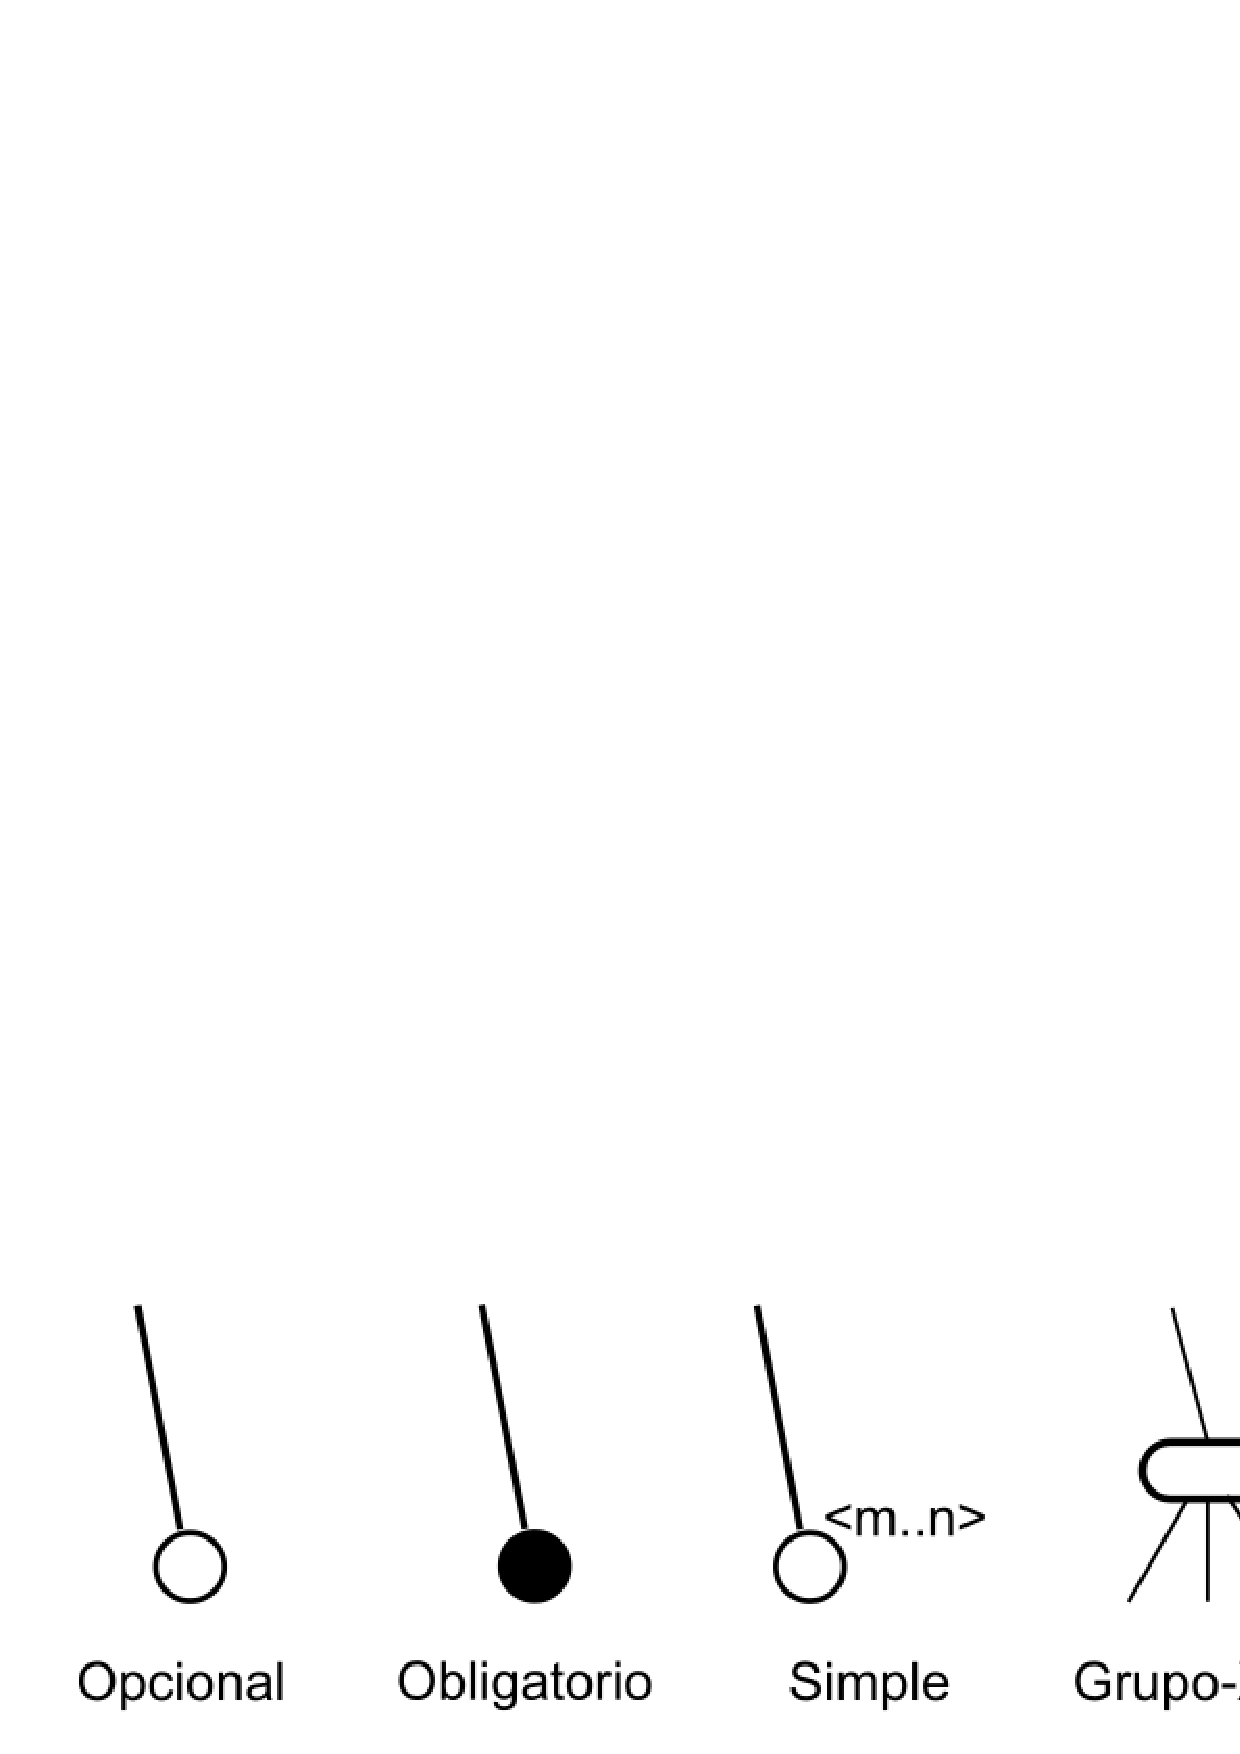
\includegraphics[scale=0.35]{background/relations.jpg}
\caption{Distintos tipos de relaciones en un modelo de caracter�sticas }
\label{fig6}
\end{figure}

1 - Opcional: La caracter�stica hija puede estar o no estar seleccionada
2 - Obligatoria: La caracter�stica es requerida.
3 - Simple: La caracter�stica tendr� una cardinalidad <m,n>, siendo m y n n�meros enteros que denotan el m�nimo y el m�ximo respectivamente de caracter�sticas que podemos seleccionar.
4 - Grupo-xor: S�lo una de las caracter�sticas pertenecientes al grupo ser� seleccionada.
5 - Grupo-or: Podremos seleccionar como m�nimo una de las subcaracter�sticas, y como m�ximo todas.
6 - Grupo simple: El n�mero de caracter�sticas seleccionadas del grupo vendr� dado por su cardinalidad <m,n>.

Adem�s se podr�n disponer de restricciones de usuario m�s complejas, que son las que se han implementado en el editor de especificaci�n y validaci�n de restricciones desarrollado en este proyecto.

\begin{figure}[t]
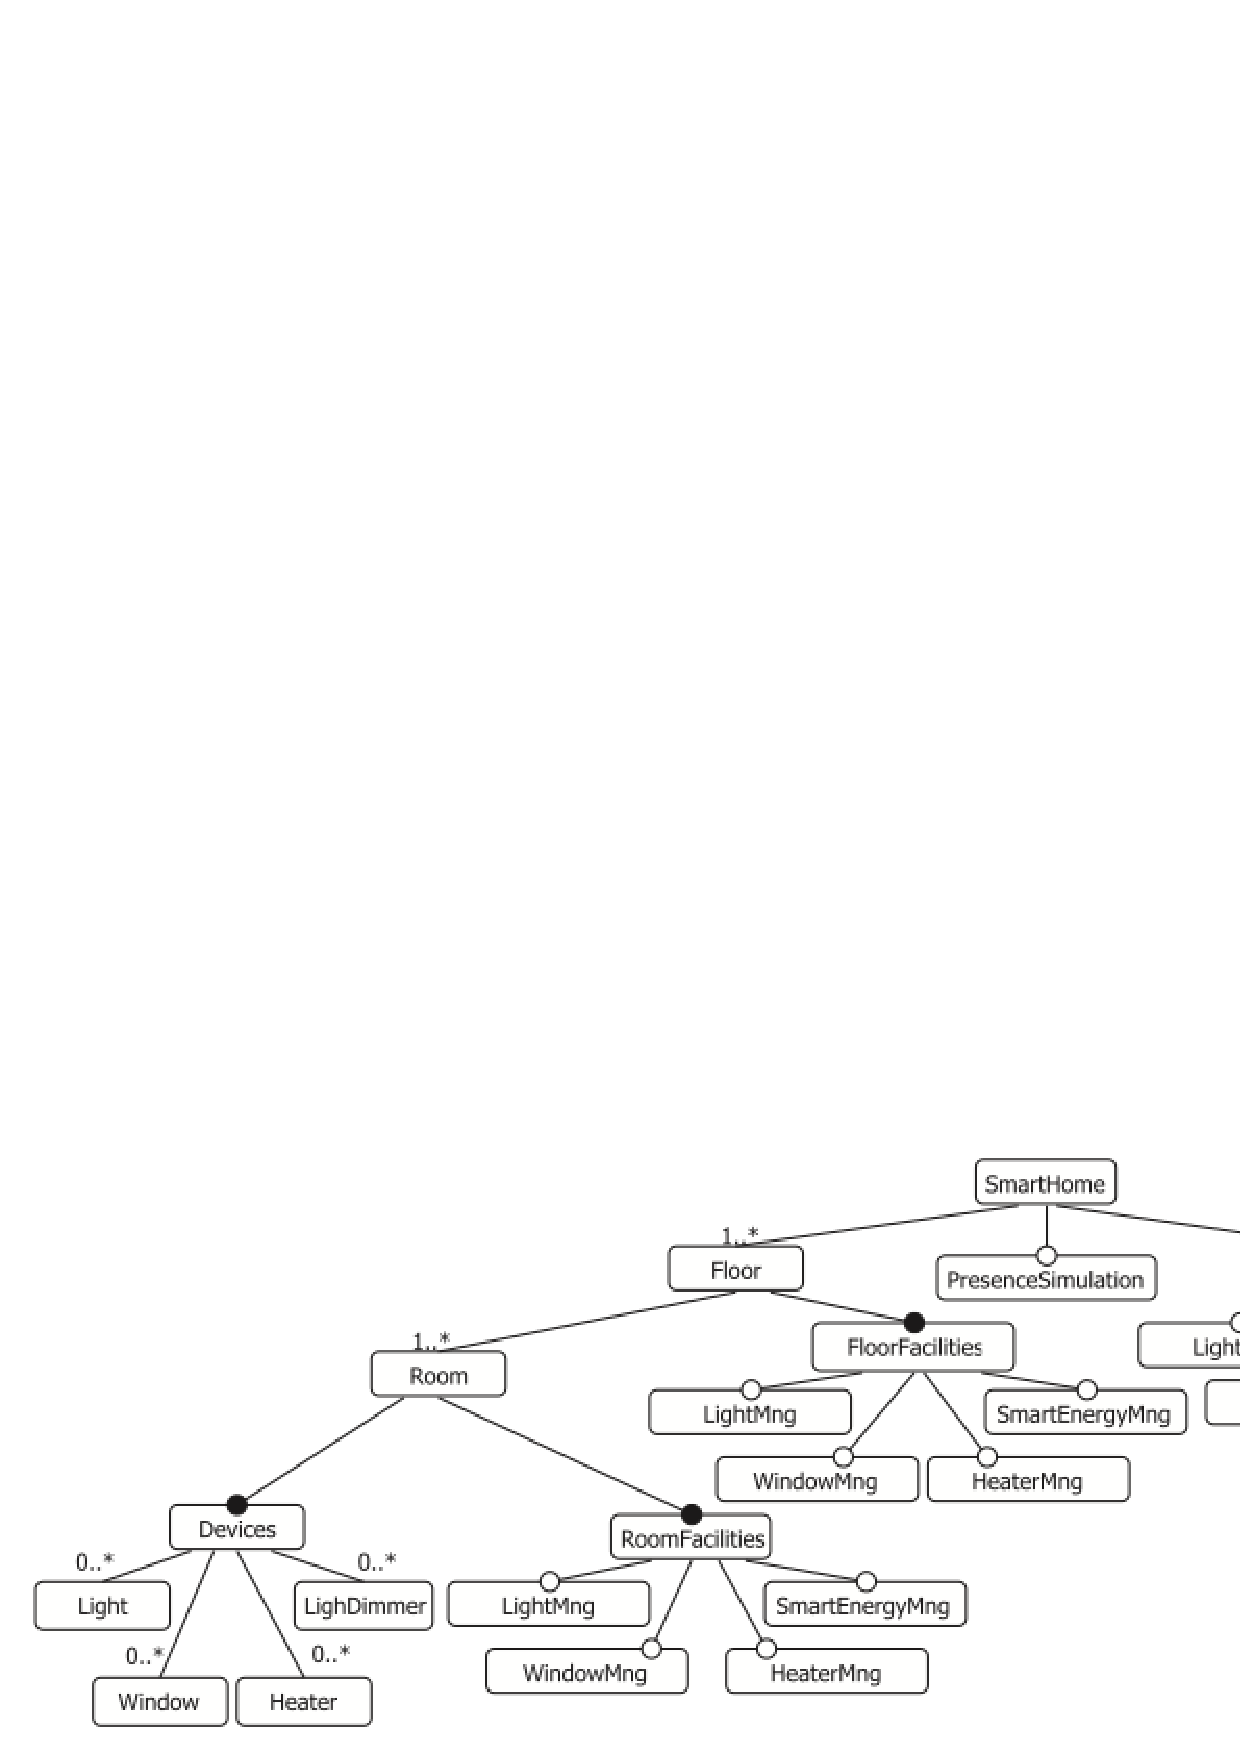
\includegraphics[scale=0.5]{background/featuremodel.jpg}
\caption{�rbol de caracter�sticas para crear una SmartHome }
\label{fig7}
\end{figure}

La figura \ref{fig7} muestra un ejemplo de modelo de caracter�sticas. En este caso se trata de un modelo de una casa inteligente o SmartHome, a trav�s del cual, seleccionando ciertas caracter�sticas u otras podremos construir qu� tipo de casa queremos. Cada una de las m�ltiples casas diferentes que podamos construir es lo que se denonima una especializaci�n o configuraci�n de nuestro modelo de caracter�sticas.

El proceso de crear una configuraci�n a partir de un modelo de caracter�sticas se conoce como proceso de configuraci�n o proceso de especializaci�n. Consiste en transformar un modelo de caracter�sticas de tal forma que el modelo resultante sea un subconjunto de las posibles configuraciones denotadas por el primer modelo. La figura \ref{fig8} muestra una posible configuraci�n para el modelo de caracter�sticas de la figura \ref{fig7}.

\begin{figure}[t]
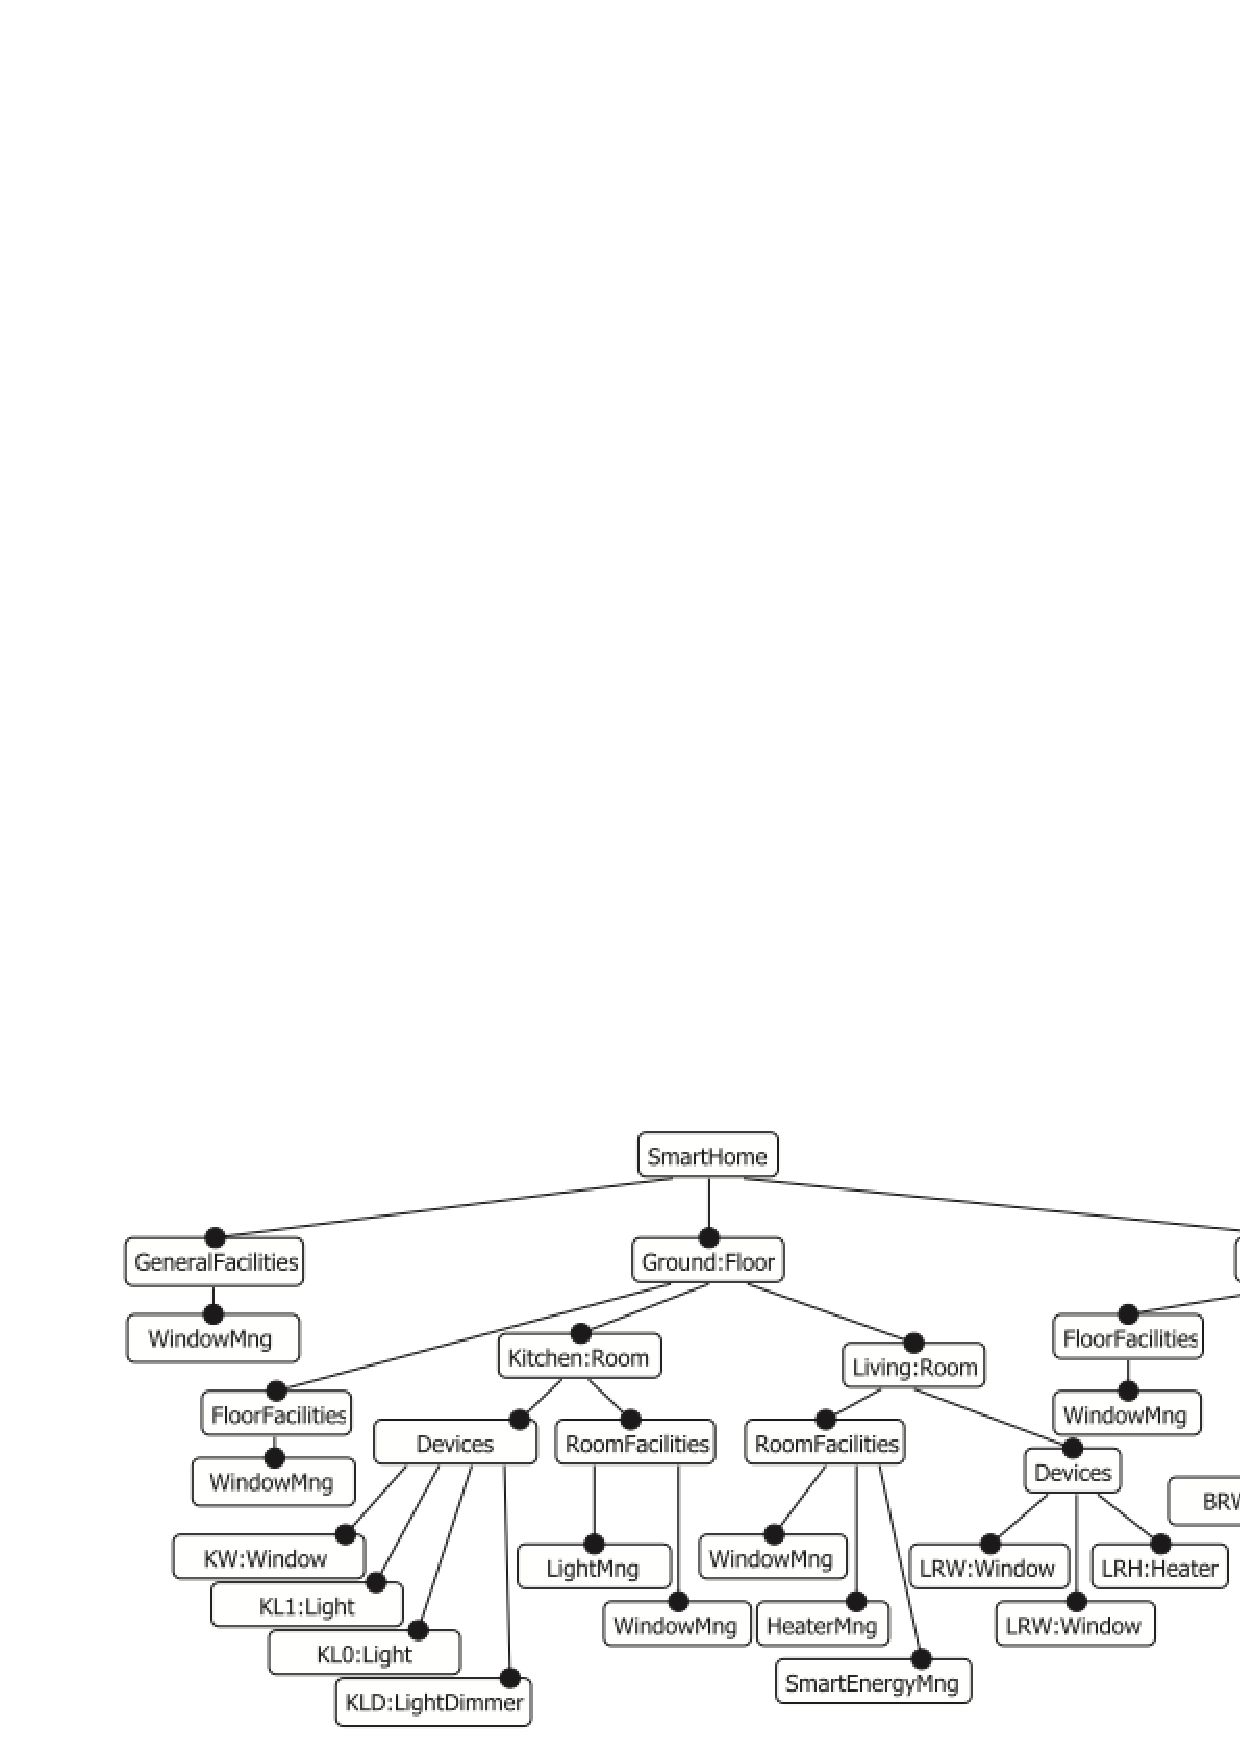
\includegraphics[scale=0.5]{background/configuration.jpg}
\caption{Especializaci�n del modelo de la figura \ref{fig7}, que representa una de las posibles casas que se pueden construir }
\label{fig8}
\end{figure}

La relaci�n entre un diagrama de caracter�sticas y una configuraci�n es an�loga a la existente entre una clase y una de sus instancias en programaci�n orientada a objetos.







\section{\emph{Eclipse Modelling Framework}}
\label{sec:back:ecore}
%%==================================================================%%
%% Author : Tejedo Gonz�lez, Daniel                                 %%
%%          S�nchez Barreiro, Pablo                                 %%
%% Version: 1.0, 18/11/2012                                         %%                  
%%                                                                  %%
%% Memoria del Proyecto Fin de Carrera                              %%
%% Antecedentes, ecore                                              %%
%%==================================================================%%

EMF \emph{Eclipse Modeling Framework}~\cite{steinberg:2008} es un \emph{plug-in} para Eclipse~\cite{clayberg:2008} que permite elaborar metamodelos. Pera ello proporciona un lenguaje de metamodelado denominado Ecore, el cual se ha convertido en el est�ndar \emph{de facto} para la realizaci�n de metamodelos. Utilizando Ecore se pueden crear metamodelos de forma gr�fica usando una notaci�n muy similar a la los diagramas de clases de UML. La Figura~\ref{fig:sle:metamodeloGrafo} muestra un sencillo ejemplo de metamodelo en Ecore (ver Secci�n~\ref{sec:intr:sle} para m�s detalles). EMF tambi�n incorpora una herramienta para la validaci�n reglas adicionales que no puedan ser especificadas a nivel de del metamodelo. 
 
EMF permite que, a partir de un metamodelo especificado en Ecore, podamos, utilizando diversos generadores de c�digo, crear autom�ticamente un conjunto de clases que nos permiten manipular dichos modelos a nivel de c�digo. Dichas clases se pueden adem�s distribuir como \emph{plug-in} para el entorno Eclipse.

Adem�s, al haberse convertido en est�ndar \emph{de facto} para el desarrollo de metamodelos, Ecore es compatible con multitud de herramientas para Ingenier�a de Lenguajes Dirigida por Modelos, como EMFText, la cual se describe en la siguiente secci�n, o diversos generadores de c�digo o herramientas de transformaci�n de modelos. 



\section{EMFText}
\label{sec:back:emftext}
%%==================================================================%%
%% Author : Tejedo Gonz�lez, Daniel                                 %%
%%          S�nchez Barreiro, Pablo                                 %%
%% Version: 1.0, 18/11/2012                                         %%
%% Version: 2.0, 06/02/2013                                         %%
%%                                                                  %%
%% Memoria del Proyecto Fin de Carrera                              %%
%% Antecedentes, emftext                                            %%
%%==================================================================%%


EMFText~\cite{emftext:2009} es una herramienta para dise�ar sintaxis textuales para metamodelos Ecore, siguiendo un enfoque de Ingenier�a de Lenguajes Dirigida por Modelos. Utilizando EMFText podemos definir la sintaxis textual de un lenguaje software utilizando una notaci�n similar a las de las notaci�n BNF. La Figura~\ref{fig:sle:gramaticaGrafos} muestra un ejemplo de gram�tica definida en EMFText para el lenguaje de grafos presentado en la Secci�n~\ref{sec:intr:sle}. 

%%==================================================================%%
%% NOTA(Pablo): Aqu� haz una gram�tica en EMFText para el lenguaje  %%
%%              de grafos del Cap�tulo 1                            %%
%%==================================================================%%

\begin{figure}[!tb]
    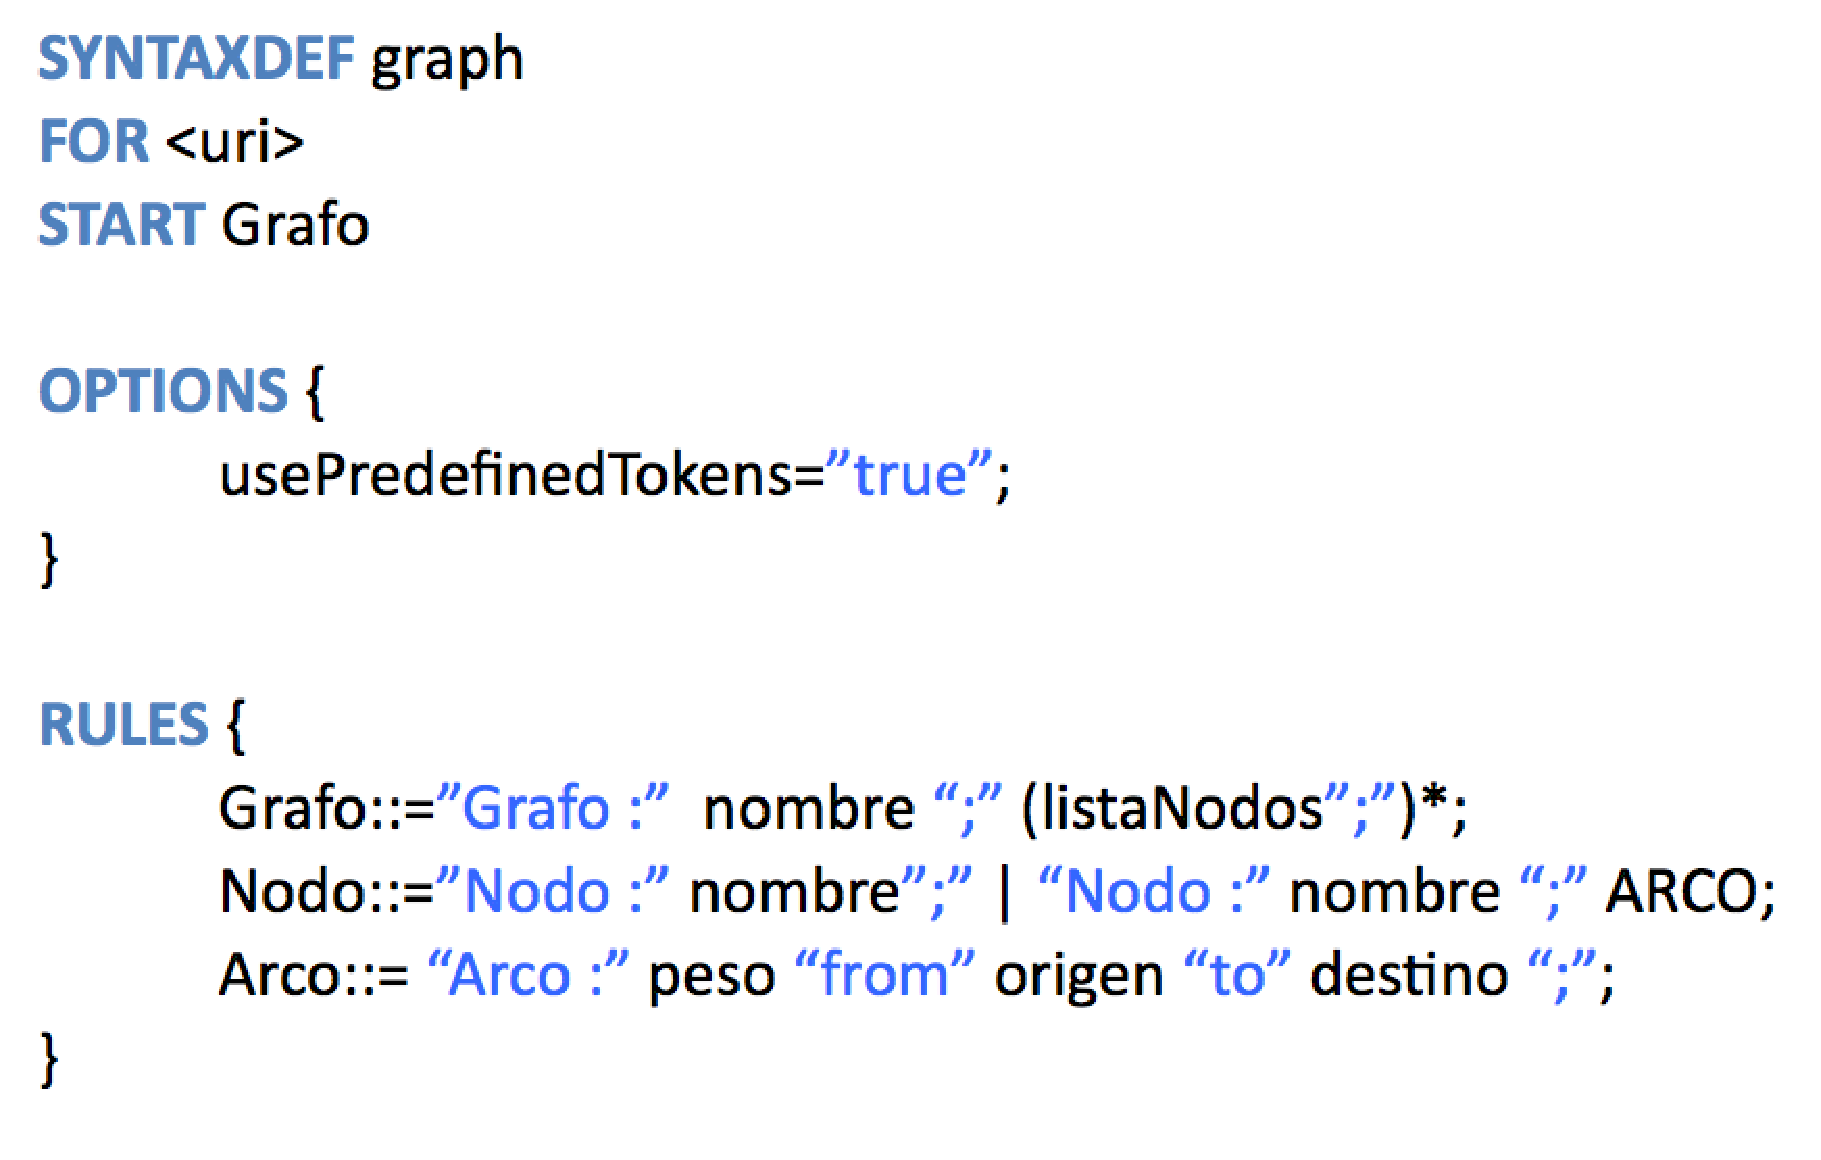
\includegraphics[scale=0.25]{background/gramaticaGrafo.eps}
    \caption{Gram�tica para el ejemplo del lenguaje de los grafos}
    \label{fig:sle:gramaticaGrafos}
\end{figure}

La sintaxis de EMFText difiere de las sintaxis BNF en que existen una serie de directivas para asociar elementos de la sintaxis textual con metaclases, de forma que se generen instancias de dichas metaclases a medida que se procesa el c�digo de un modelo. Por ejemplo, tal y como est� definida la gram�tica de la Figura~\ref{fig:sle:gramaticaGrafos}, a medida que vamos definiendo los arcos estamos indicando la informaci�n tanto de su peso como de sus nodos origen y destino. De este modo, EMFText genera una instanciaci�n de la metaclase Arco que inicializa con los datos le�dos y la a�ade a la instancia global del metamodelo.

La gran ventaja de EMFText es permite generar, a partir de la definici�n de una gram�tica, una gran cantidad de c�digo, liberando al programador de tareas tediosas que adem�s en muchos casos podr�an resultar complicadas. Utilizando EMFText se puede generar autom�ticamente: (1) un editor para nuestro lenguaje, con facilidades como coloreado de la sintaxis o autocompletado; (2) un procesador para el lenguaje capaz de generar una instancia de su correspondiente metamodelo; y (3) el c�digo necesario para empaquetar y distribuir dicho editor como un \emph{plug-in} para Eclipse. Adem�s, todo el c�digo generado es completamente independiente de EMFText, por lo que puede ser ejecutado en plataformas que no tengan instalado dicha herramienta; y es personalizable. Por ejemplo, se puede modificar f�cilmente el postprocesador de nuestra gram�tica. 






\section{Arquitectura de plugins de Eclipse}
\label{sec:back:eplugins}
%%==================================================================%%
%% Author : Tejedo Gonz�lez, Daniel                                 %%
%%          S�nchez Barreiro, Pablo                                 %%
%% Version: 1.0, 18/11/2012                                         %%                   
%% Version: 1.0, 06/02/2013                                         %%                   
%%                                                                  %%
%% Memoria del Proyecto Fin de Carrera                              %%
%% Antecedentes, arquitectura de plugins de eclipse                 %%
%%==================================================================%%

En entorno de desarrollo Eclipse es un ejemplo de arquitectura modular f�cilmente extensible mediante una compleja, pero sencilla al programador, arquitectura de \emph{plug-ins}. Un \emph{plug-in} en Eclipse es un componente que provee un cierto tipo de servicio dentro del contexto del espacio de trabajo de Eclipse. Es decir, una herramienta que se puede integrar en el entorno Eclipse junto con sus otras funcionalidades. Dado que la herramienta \emph{Hydra} fue dise�ada como un \emph{plug-in} para Eclipse, y nuestro editor pretende integrarse tanto en \emph{Hydra} como en \emph{Eclipse}, es necesario conocer y manejar el funcionamiento de la arquitectura de plug-ins de Eclipse.

%%==============================================================================================%%
%% NOTA(Pablo): Esto no se entiende nada
%%==============================================================================================%%
%%
%% En particular, se han utilizado mucho los puntos de extensi�n. Un punto de extensi�n en un
%% plug-in indica la posibilidad de que ese plug-in sea a su vez parte de otro, o que haya 
%% otros plug-ins que sean parte de �l. Esta particularidad permite no s�lo la integraci�n de 
%% nuestro editor con Hydra, sino tambi�n la personalizaci�n de men�s y botones para �l 
%% gracias a la creaci�n de puntos de extensi�n con plug-ins de creaci�n de men�s y barras de
%% herramientas.
%%
%%==============================================================================================%%

%%==============================================================================================%%
%% NOTA(Pablo): Para solucionar
%% - Describir en uno o dos p�rrafos c�mo funciona la arquietctura de plug-ins para Eclipse
%% - Poner un ejemplo de punto de extensi�n, sencillo y concreto, y explicar como funciona 
%%   el punto de extensi�n utilizando algo de c�digo.
%% Si no sabes como escribir esta secci�n, la eliminas directamente, y actualizas la intro 
%% al Cap�tulo de forma conveniente.
%%==============================================================================================%%


\section{Sumario}
\label{sec:back:sumario}
\todo{Escribe un peque�o sumario para el cap�tulo}
% %%==================================================================%%
%% Author : Tejedo Gonz�lez, Daniel                                 %%
%%          S�nchez Barreiro, Pablo                                 %%
%% Version: 1.0, 25/11/2012                                         %%                   
%%                                                                  %%
%% Memoria del Proyecto Fin de Carrera                              %%
%% Sintaxis abstracta, sumario                          %%
%%==================================================================%%

Durante el presente cap�tulo se ha descrito el proceso de definici�n de la sintaxis abstracta de nuestro lenguaje. Este proceso abarca subtareas como la captura de requisitos del lenguaje, la creaci�n de un metamodelo que permita la creaci�n de sintaxis concretas apropiadas, la validaci�n de restricciones externas a ese metamodelo, y las pruebas que corroboren que todos los elementos creados funcionan correctamente. En el siguiente cap�tulo profundizaremos acerca del dise�o de la gram�tica para nuestro lenguaje, as� como de las herramientas utilizadas para implementar esa gram�tica.


% Cap�tulo 3: Descripci�n General del Proceso
\todo{Cap�tulo 3: Alcance y Planificaci�n del Proyecto}

% Cap�tulo 4: Ingenier�a de Requisitos
\todo{Cap�tulo 4: Ingenier�a de Requisitos}

% Cap�tulo 5: Definici�n Arquitect�nica y Dise�o Software
\todo{Cap�tulo 5: Definici�n Arquitect�nica y Dise�o Software}

% Cap�tulo 6: Construcci�n e Implementaci�n
\todo{Cap�tulo 6: Construcci�n e Implementaci�n

% Cap�tulo 7: Pruebas, Despliegue y Aceptaci�n
\todo{Cap�tulo 7: Pruebas, Despliegue y Aceptaci�n}

% Cap�tulo 8: Discusi�n, Conclusiones y Trabajos Futuros
\todo{Cap�tulo 7: Discusi�n, Conclusiones y Trabajos Futuros}

% CONTENT: Appendices, if desired
\renewcommand\chaptername{Appendix}                      % hereafter, chapters are called "Appendix"
\renewcommand\thechapter{\Alph{chapter}}        % chapter number in Romans
\renewcommand\thesection{\Alph{chapter}.\alph{section}}  % make sections "I.a", instead of "1.1"
\setcounter{chapter}{0}                                  % start numbering chapters from 1 on again


% Appendix A:
% \input{populo/populo.tex} % Appendix I

% CONFIG: Bibliography style
% \cleardoublepage                            % start in right side page
\addcontentsline{toc}{chapter}{References}  % add this "chapter" to the ToC, with the name "Bibliography"
%\bibliographystyle{alpha}                  % bibliography style
\bibliographystyle{abbrv}                  % bibliography style
% \bibliography{references/references}

\end{document}
